
\chapter{Chapter 2 Supplemental Information}
\label{sec:app2}
\raggedbottom

{\let\thefootnote\relax\footnotetext{This chapter was originally published as Braun, C.D., Galuardi, B., and Thorrold S.R. (2018). \href{http://onlinelibrary.wiley.com/doi/10.1111/2041-210X.12959/full}{HMMoce: An R package for improved geolocation of archival-tagged fishes using a hidden Markov method.} \emph{Methods in Ecology and Evolution} 9, 1212-1220. }}
%\end{singlespace}
{\let\thefootnote\relax\footnotetext{C.D.B and B.G. conceived the project and developed the package; C.D.B and S.R.T. collected the data; C.D.B. wrote the paper; B.G. and S.R.T. contributed to the writing of the paper.}}

\clearpage

\section{Supplemental Methods}

\subsection{The Approach}

We present a state-space model to estimate movements and behavior from uncertain and temporally correlated oceanographic data collected with electronic tags. Estimation of unknown states (movements and behavior) based on observations is formulated as a hidden Markov model (HMM) on a spatial grid in continuous time. While many details set \texttt{HMMoce} apart from other HMM methods for electronic tag data, the logic of the underlying approach is similar and discussed in detail elsewhere \citep{Pedersen2008, Pedersen2011, Thygesen2009a}. A key feature of \texttt{HMMoce} and its predecessors is the discretization of space over a grid. In this manner, location estimation can be supplemented by, or based entirely on, environmental data (\eg sea surface temperature or oceanographic profiles).

The logic and use of \texttt{HMMoce} is as follows: 
\begin{enumerate}[itemsep=-1mm]
    \item prepare tag data and acquire necessary environmental data
    \item calculate gridded likelihoods based on observations
    \item form the model
    \item get movement parameters
    \item finalize track and space use metrics
\end{enumerate}

\subsection{Data preprocessing}%\label{sec:prep}

The \texttt{HMMoce} package contains several custom routines for reading and formatting Wildlife Computers tag data that can then be leveraged in the observation portion of the model (refer to package vignette for data requirements). Currently, light-based position estimates (GPE2), with manual filtering of clearly spurious positions, are used to define the temporal and spatial limits of interest; but this may be overridden by the user. After tag data preparation, gridded environmental data (\emph{e.g.} sea surface temperature, SST) is acquired from various online repositories. Gridded monthly climatological mean depth-temperature data from the World Ocean Atlas 2013 (WOA, 0.25$^{\circ}$ resolution), daily reanalysis model depth-temperature products from the HYbrid Coordinate Ocean Model (HYCOM, 0.08$^{\circ}$ resolution) and daily optimally interpolated sea surface temperature fields (OI-SST, 0.25$^{\circ}$ resolution) are acquired using \texttt{get.env} and the appropriate \texttt{type} argument. See \texttt{HMMoce} package documentation (\texttt{?get.env}) for more details on environmental data and for options to use additional input datasets.

\subsection{Calculating likelihoods}%\label{sec:lik}

Likelihoods are calculated using light-based longitude estimates, SST and depth-temperature profiles (collected by the archival tag). For each time point, $t$ (here we use daily), we calculate a likelihood of the animal's position ($L(x_{(t)})$) on the grid:

\begin{equation}
L(x_{(t)}) = L(x_{(t)})_1 \times L(x_{(t)})_2 \times ... L(x_{(t)})_n
\label{eq:a1e1}
\end{equation}

where 1:$n$ indicates individual likelihood components, which are formed for each type of input data at each time point (\textit{e.g.} $L_{SST}(x_{(t)})$). Currently, \texttt{HMMoce} is built for n $\leq$ 3 because no combination of light, SST and depth-temperature profiles can sensibly be combined for n $>$ 3 (\emph{i.e.} cannot use both WOA and HYCOM likelihood at the same time).

\subsubsection{Light-based longitudinal
likelihoods}%\label{light-based-longitudinal-likelihoods}

Tags record light levels from which sunrise and sunset times can be calculated \citep{Hill2001}. We calculate position estimates using Wildlife Computers GPE2 software, which allows vetting of spurious light measurements. The longitude and corresponding error estimate from GPE2 are used to evaluate a probability density function, resulting in a likelihood surface for this data. \texttt{HMMoce} also includes functionality for using latitude estimates (resulting in elliptical likelihood surfaces), but the default is longitude only.

\subsubsection{SST likelihoods}

For daily SST likelihoods, we construct a probability density function integrated between calculated limits \citep{LeBris2013a} to incorporate observational errors (e.g.~tag sensor error and/or near-surface SST measurements). We form a daily SST likelihood by integrating between limits for tag-measured SST ($SST_{min},SST_{max}$) that encompasses the range of SST values (including observation error) measured within that day:

\begin{equation}
L_{SST}(x_{(t)}) = \int_{SST_{min}}^{SST_{max}} N(t; \mu_z, \sigma_z)~dz
\label{eq:a1e2}
\end{equation}

where $N$ is a normal probability distribution function, $\mu_z$ the remotely-sensed SST grid cell value, and $\sigma_z$ the grid cell standard deviation. Standard deviation for remotely-sensed SST values are calculated using a "moving window" mean from \texttt{raster::focal} in \texttt{R} to incorporate approximately 0.25$^{\circ}$ of SST data around each cell.

\subsubsection{Profile-based
likelihoods}

Archival tags collect summaries of depth-temperature profiles at user-defined intervals throughout the deployment period. While these summaries vary in temporal and spatial resolution depending on study species, the profiles are a representation of a particular environment and time point during tag deployment that can be exploited in a spatial context. Tag profile data is recorded at various depth levels that often does not correspond to standard depth levels produced for the World Ocean Atlas or HYCOM. Thus, in all cases, we use linear regression in the \texttt{R} package \texttt{locfit} to predict profile temperatures from the tag at standard oceanographic depth levels in the corresponding dataset of interest. In addition, Wildlife Computers tags collected daily minimum and maximum temperatures at all depth levels which yield a thermal envelope of possible temperatures (rather than a single profile). In all cases, we construct a probability density function integrated between calculated limits \citep{LeBris2013a} (\emph{e.g.} minimum and maximum temperature), and standard deviation is calculated using a "moving window" as described previously for SST likelihood. Likelihoods based on tag profile data can be constructed using 3 different approaches.

\paragraph{Ocean Heat Content}%\label{ocean-heat-content}

Ocean heat content (OHC) is an integrated measure of temperature in the upper ocean that has been used by oceanographers and meteorologists since the mid-20th century \citep{Palmen1948} and may reveal complex structuring in the upper ocean at the mesoscale \citep{Luo2015}. OHC is calculated by integrating the thermal energy above an isotherm depth ($D$) to the surface as:

\begin{equation}
OHC = c_p\rho\int_{D}^{0} (T_z - T_D)~dz
\label{eq:a1e3}
\end{equation}

where, $c_p$ is the specific heat constant of water (3.993 $\frac{kJ}{kg}~C$), $\rho$ is sea water density (1025 $\frac{kg}{m^3}$), $T_z$ is water temperature ($^{\circ}$C) at depth $z$ and $T_D$ is water temperature at isotherm depth $D$. This results in a single minimum and maximum OHC metric for each day of tag profiles (see min/max discussion above) between which a probability density function is integrated to incorporate the range of possible tag-based OHC values. OHC calculations are performed on daily 0.08$^{\circ}$ HYCOM grids which form the environmental grids used to compare tag observations to in the probability density framework:

\begin{equation}
L_{OHC}(x_{(t)}) = \int_{OHC_{min}}^{OHC_{max}} N(t; \mu_z, \sigma_z)~dz
\label{eq:a1e4}
\end{equation}

where $N$ is a normal probability distribution function, $\mu_z$ the OHC grid cell value calculated from a daily HYCOM grid and $\sigma_z$ the grid cell standard deviation.

\paragraph{World Ocean Atlas and
HYCOM}%\label{world-ocean-atlas-and-hycom}

The World Ocean Atlas 2013 contains a climatological monthly mean temperature for the global ocean from in situ profile data on a 1/4$^{\circ}$ or 1$^{\circ}$ grid \citep{Locarnini2013}. Tag-based minimum and maximum temperature profiles (after regression to predict values at standard WOA depth levels) are compared to WOA grids at standard depth levels to generate a likelihood surface at individual depth levels, $n$:

\begin{equation}
L_{WOA}(x_{(t)})_n = \int_{T_{min_n}}^{T_{max_n}} N(t; \mu_z, \sigma_z)~dz
\label{eq:a1e5}
\end{equation}

where $N$ is a normal probability distribution function, $\mu_z$ the WOA grid cell temperature at depth $n$ and $\sigma_z$ the temperature standard deviation at depth $n$. Then the product of likelihood surfaces at each depth level (1:$n$) is calculated to generate a single depth-temperature profile likelihood for time $t$:

\begin{equation}
L_{WOA}(x_{(t)}) = L_{WOA}(x_{(t)})_1 \times L_{WOA}(x_{(t)})_2 \times ... L_{WOA}(x_{(t)})_n  
\label{eq:a1e6}
\end{equation}

The same process is repeated to calculate depth-temperature profile likelihoods using HYCOM as the environmental grid to formulate $L_{HYCOM}(x_{(t)})$.

\subsection{Model formulation}%\label{sec:model}

Details of model formulation, estimation and selection for \texttt{HMMoce} are derived from \citet{Pedersen2011} and are discussed there in depth. Briefly, the movement of an animal is considered as a Brownian motion which, given the current behavior state $I_t$ of the animal, is decribed by a diffusivity matrix $D_{I_t}$ with unit km$^2$ day$^{-1}$. The application of diffusion processes in animal movement modeling is well established for analysis of tag data \citep[e.g.][]{Sibert2003, Pedersen2008} and more broadly \citep{Okubo2013}. We consider the joint process of movement and behavioral states as a probability density $\varphi_i(x,y,t)$ which describes the probability that the animal at time $t$ is located at $(x, y)$ and is in behavioral state $i$. The time evolution of the probability density of a particle performing brownian motion follows a diffusion-advection equation which can be augmented to include behavior switching dynamics \citep[see Eqn. 1,][]{Pedersen2011a}. Our approach uses numerical approximation to solve an advection-diffusion equation by discretizing the continuous state-space into a grid \citep{Thygesen2009a}. In discrete state-space, the probability density can be represented by a vector, $\varphi$, containing the state probabilities $(x,y,i)$ through time.

Model estimation is conducted in a HMM framework using a filtering approach \citep{Zucchini2009} that yields the probability distribution of states moving forward in time conditional on observations, $\varphi(t_k | Z_k)$. The filter recursion alternates between time and data updates and returns a likelihood measure that can be used for parameter estimation and model selection. The final step includes a HMM smoothing step \citep{Thygesen2009a} that works backwards in time on filtered state estimates, thus leveraging the full dataset. This step provides the posterior probability distribution of each state (\eg location and behavior) at specific times (typically daily). For more details on model formulation, see \citet{Pedersen2008} and \citet{Pedersen2011a} and references therein.

Most of the HMM filtering and smoothing mechanics remain unchanged from that developed by \citet{Pedersen2008}; however, two main improvements are worth noting. First, image processing techniques are used in the convolution steps at each time point in the filter (see \texttt{?hmm.filter}) to make the convolution more intuitive and improve computation speed. For full details of the convolution, see \texttt{?imager::convolve} \citep{Barthelme2016}. Second, we add a masking technique within the filtering step that allows the user to set boundary thresholds on how much of the observation likelihood grid is used in the filter step. This masking approach can be used to set a constant distance, or a percent threshold of the bounding box, from the previous day's output to help constrain the following day's results. This approach is still experimental but may help constrain position estimates by weighting regions of the observation likelihood more highly if they are closer to the previous days filter probability.

\subsubsection{Parameter Estimation}%\label{sec:param}

The filtering process above returns a likelihood measure which indicates how well the model fits the data. Thus, this likelihood function of the unknown parameters $\theta$ (\emph{e.g.} diffusion, switching rates) can be evaluated at, say, $\theta_0$ by running the filter using the parameter values in $\theta_0$. Maximum likelihood (ML) estimation of model parameters is then straight forward and can be performed by most standard numerical optimizers. However, recent work by \citet{Woillez2016} further exploited the properties of the discretization of space in this model and addressed a joint ML estimation of all model parameters using an iterative Expectation-Maximization (EM) framework.

Here the EM algorithm is a two-step iterative procedure: the expectation (E) step computes the posterior distribution $P((X_t)_{t=0:N-1} | (Y_t)_{t=0:N-1})$ given current model parameter estimates, $\theta_v$; and the maximization (M) step updates model parameters ($\theta_{v+1}$) according to a ML criterion reweighted by the posterior distribution. Currently in \texttt{HMMoce}, $\theta_v$ represents transition probability between states, while movement parameters are fixed to realistic estimates of diffusion as determined by estimated tag speeds calculated from Argos-based positions or based on expert knowledge. The theoretical movement process is considered purely Brownian, and advection is currently not considered. The two-step EM procedure for state-switching probabilities is iterated through $\theta_N$ until a convergence threshold is met. Switching rates are calculated in an EM framework following \citet{Woillez2016} (see \texttt{expmax} function in \texttt{HMMoce}) with a change threshold that defaults to 1\%.

\subsubsection{Model results}%\label{sec:track}

There are a number of ways the posterior distribution of the state can be used to represent animal movements. Approaches in the literature have been to calculate the mean or mode across the distributions through time \citep{Pedersen2008, Pedersen2011a} to represent a most probable track. A third approach to estimate most probable tracks from the posteriors is using the Viterbi algorithm \citep{Viterbi2006} which has been used in movement ecology \citep{Pedersen2008, Thygesen2009a, Winship2012, Jonsen2013} but is extremely computationally intensive. \texttt{HMMoce} currently has functionality for both mean and mode.

Summing the posterior distribution over time across all behaviors yields a distributional estimate of residence time \citep{Pedersen2011a} as well as yields insight on the cumulative distribution of the animal's residency (utilization distribution). Similarly, behavior state estimates can be summed over space to get the probability of the animal being in each behavioral state through time and across the recorded movements and can be used to detect differential space use (\emph{e.g.} \cref{fig:c2f4} in the main text).

\subsection{Case study methods}%\label{case-study-methods}

\subsubsection{Tagging methodology}%\label{tagging-methodology}

Three blue sharks and one shortfin mako were tagged near Cape Cod, MA during Fall 2015 with both pop-up satellite archival transmitting (PSAT) tags and Argos-based SPOT tags. Sharks were caught on rod and reel and then brought onboard the fishing vessel. We attached satellite-linked radio telemetry tags (Wildlife Computers finmount SPOT5 tags) to the dorsal fin with nylon surgical hardware. PSAT tags were attached to a short (\textless{}20 cm) stainless steel tether that terminated in a titanium anchor. The anchor was inserted into the dorsal musculature near the base of the dorsal fin. PSATs were programmed to report summarized daily depth-temperature profiles, sunrise and sunset event timing and sea surface temperature and to pop-up 180 days after tagging. The SPOT tag collected Doppler-based geopositions from Argos satellites when a wet/dry switch on the tag was activated at the surface-air interface. Resulting locations were processed with a Kalman filtering algorithm by Collecte Localisation Satellites \citep{Lopez2014} and subsequently assigned error flags called location classes (LC): LC 3, \textless{}250 m; LC 2, 250-500 m; LC 1, 500-1500 m; LC 0, \textgreater{}1500 m for classes 3, 2, 1, 0. Additional classes A, B represented positions derived from less than 4 satellite messages and were not assigned an estimated spatial accuracy. Location class Z positions were considered invalid and removed from further analysis \citep{CLS2016}. After Z class positions were removed, the remaining positions were filtered using a speed filter (2 $m s^{-1}$) from the \texttt{trip} package \citep{Sumner2015}, based on characteristic speeds (\cref{fig:a1f1}), and regularized to daily positions using \texttt{crawl} \citep{Johnson2008a} in \texttt{R} \citep{RDevelopmentCoreTeam2015}. Results metrics from various \texttt{HMMoce} model runs (referred to in the main text) are shown in Table \ref{tab:a1t1}. One complete blue shark dataset is included as example data in the package, and its analysis is described in full detail in the package vignette.

\subsubsection{Grid resolution and time
trials}%\label{grid-resolution-and-time-trials}

Our method uses grid-based computations as they afford both flexibility and computational improvements, but changes in grid size can alter likelihood surfaces, model results and computation time. Several trials of \texttt{HMMoce} were conducted on an Amazon EC2 instance (2.3 GHz Intel Xeon processors, 64 CPUs, 256 GiB memory) and a consumer grade desktop computer (2.53 GHz processors, 4 CPUs, 12 GiB memory) encompassing various grid sizes. \texttt{HMMoce} modeling was initially performed on 0.25$^{\circ}$ grids, including likelihoods and model selection, to match the grid-based calculations conducted in GPE3 \citep{WC2015}, but the resolution was increased to a 0.08$^{\circ}$ grid for the final model runs for each tag dataset. Results from time trial and grid resolution model runs indicated that higher resolution grids (as fine as 0.08$^{\circ}$) yielded roughly equivalent results to slightly more coarse (0.25$^{\circ}$) grids while significantly increasing computation time (approx. 3-fold increase) (Table \ref{tab:a1t2}). However, grids as coarse as 1$^{\circ}$ often yielded poor fit metrics (10-fold increase in error), likely as a result of the loss of mesoscale variability in oceanographic data at this resolution.

\subsubsection{Data removal experiment}%\label{data-removal-experiment}

While \texttt{HMMoce} was designed to improve geolocation estimates for all tagged marine organisms, the main impetus for the work was to fulfill a need for improving track estimates in cases where light and SST data (from minimal surface occupation) were lacking. In order to use the double-tagged shark dataset (with high quality light and SST data) to test this, we randomly removed (using \texttt{sample} in base \texttt{R}, without replacement) 75\% and 50\% of deployment days with adequate light and SST data, respectively, for geolocation from the shark PSAT data (while keeping the depth-temperature profile data for these days). The removals approximated PSAT data quality typical of swordfish tag deployments in the Atlantic Ocean due to crepuscular diving behavior and light avoidance \citep[][Chapter \ref{chap:2}]{Braun2015, Neilson2009}. The resulting tracks were treated as independent from track model runs performed on the complete datasets, and \texttt{HMMoce} likelihood routines and GPE3 track construction methods were unchanged.

\subsection{Other geolocation models}%\label{other-geolocation-models}

Almost all of the available geolocation approaches for archival tag data rely on light or a combination of light, SST and a bathymetric mask that is often applied ad hoc. Light-based positioning is predicated on an accurate measure of day length. Yet, many species rarely, if ever, visit the surface layer during the appropriate periods required for calculation of sunrise and sunset times \citetext{\citealp[\eg swordfish,][]{Neilson2009}; \citealp[basking sharks,][]{Skomal2009}}. Thus, we sought to develop a modeling framework that would also be applicable to species with limited light data.

To facilitate comparison of \texttt{HMMoce} with existing methods, we used two existing state-space models that have been widely used in marine biotelemetry \citep[\eg][]{Braun2015a, Galuardi2012, Lam2014, Lam2016, Thorrold2014, Winship2012}: a sea surface temperature inclusive Unscented Kalman filter, Ukfsst, \citep{Lam2008, Nielsen2007} and a coherent state-space model using raw light levels recorded on the tag, Trackit, \citep{Nielsen2007}. Sea surface temperature fields used in Ukfsst were weekly, 1$^{\circ}$ optimally interpolated values \citep{Reynolds2002}. Initial values for parameters estimated in both models were adjusted and/or flagged as inactive in the estimation until a convergence minimum was reached. A second stage bathymetric correction was applied to the estimated Ukfsst tracks to improve quality, particularly near landmasses \citep{Galuardi2010}. A global, 1$^\circ$ product, E-Topo1 \citep{Amante2009}, was used for this step. For each model estimate, the most probable track was used for comparison. While Trackit and Ukfsst are built on a fundamentally different statistical framework than the HMM models, they have been widely used in the same way to estimate movements of individuals using data from archival tag deployments. While neither Ukfsst or Trackit may have been fully optimized here, their inclusion allowed a test of the potential benefits of using 3D tag data for marine biotelemetry, particularly when quality light and SST data is lacking. We also compared our results to a proprietary, manufacturer-specific (Wildlife Computers) HMM called GPE3. The GPE3 algorithm does not permit customization of model details except "typical animal speed." Speed estimates used to generate GPE3 tracks were 2 or 4 m/s to match speeds used in \texttt{HMMoce} based on speeds of Argos-tracked sharks (\cref{fig:a1f1}). This comparison is discussed in detail in the main text. Resulting tracks from the model comparison and the \texttt{HMMoce} most probable track with behavior switching results are shown for the mako (\cref{fig:c2f2} \cref{fig:c2f3}, respectively) and the blue sharks (\cref{fig:a1f2}, \cref{fig:a1f3}, \cref{fig:a1f4}) for blue shark model comparison and \cref{fig:a1f6}, \cref{fig:a1f7}, \cref{fig:a1f8} for \texttt{HMMoce} track and behavior switching results). Discussion of model limitations and an example comparison to HYCOM, WOA and OHC likelihoods is discussed in the main text and shown in \cref{fig:a1f5}.

Reported error metrics throughout this study include great-circle distance between true (Argos) and estimated locations on the Earth's surface using the \texttt{rdist.earth.vec} function in the \texttt{fields} \citep{Nychka2015} package for \texttt{R} and root-mean-square error (RMSE) between daily model output and Argos locations \citep{Galuardi2008, Wilson2007, Braun2015a}.

\clearpage

%--------------------
%--------------------
\section{Supplemental Figures}
%--------------------
%--------------------

%Figure a1f1:
\begin{figure}[htbp]
\centering
\includegraphics[width=.7\textwidth]{images/A1_Fig1.pdf}
\caption{Density of speeds among Argos-based positions for
tagged individuals.}
\label{fig:a1f1}
\end{figure}

\clearpage

%--------------------
%Figure a1f2:
\begin{figure}[htbp]
\centering
\includegraphics[width=1\textwidth]{images/A1_Fig2.pdf}
\caption[Comparison of track methods for blue shark 141254]{Calculated tracks for blue shark 141254
using the 4 different geolocation approaches (Ukfsst, purple; Trackit,
blue; GPE3, green; \texttt{HMMoce}, yellow) compared to the ``known''
Argos-based track (red, black crosses). Latitudinal and longitudinal
estimates through time are shown in panels B and C, respectively. Lines
appear broken when a resulting track is missing daily data.}
\label{fig:a1f2}
\end{figure}

\clearpage

%--------------------
%Figure a1f3:
\begin{figure}[p]
\centering
\includegraphics[width=1\textwidth]{images/A1_Fig3.pdf}
\caption[Comparison of track methods for blue shark 141256]{Calculated tracks for blue shark 141256
using the 4 different geolocation approaches (Ukfsst, purple; Trackit,
blue; GPE3, green; \texttt{HMMoce}, yellow) compared to the ``known''
Argos-based track (red, black crosses). Latitudinal and longitudinal
position estimates through time are shown in panels B and C,
respectively. Lines appear broken when a resulting track is missing
daily data.}
\label{fig:a1f3}
\end{figure}

\clearpage

%--------------------
%Figure a1f4:
\begin{figure}[p]
\centering
\includegraphics[width=1\textwidth]{images/A1_Fig4.pdf}
\caption[Comparison of track methods for blue shark 141259]{Calculated tracks for blue shark 141259
using the 4 different geolocation approaches (Ukfsst, purple; Trackit,
blue; GPE3, green; \texttt{HMMoce}, yellow) compared to the ``known''
Argos-based track (red, black crosses). Latitudinal and longitudinal
position estimates through time are shown in panels B and C,
respectively. Lines appear broken when a resulting track is missing
daily data.}
\label{fig:a1f4}
\end{figure}

\clearpage

%--------------------

\begin{landscape}
%Figure a1f5:
\begin{figure}[p]
\centering
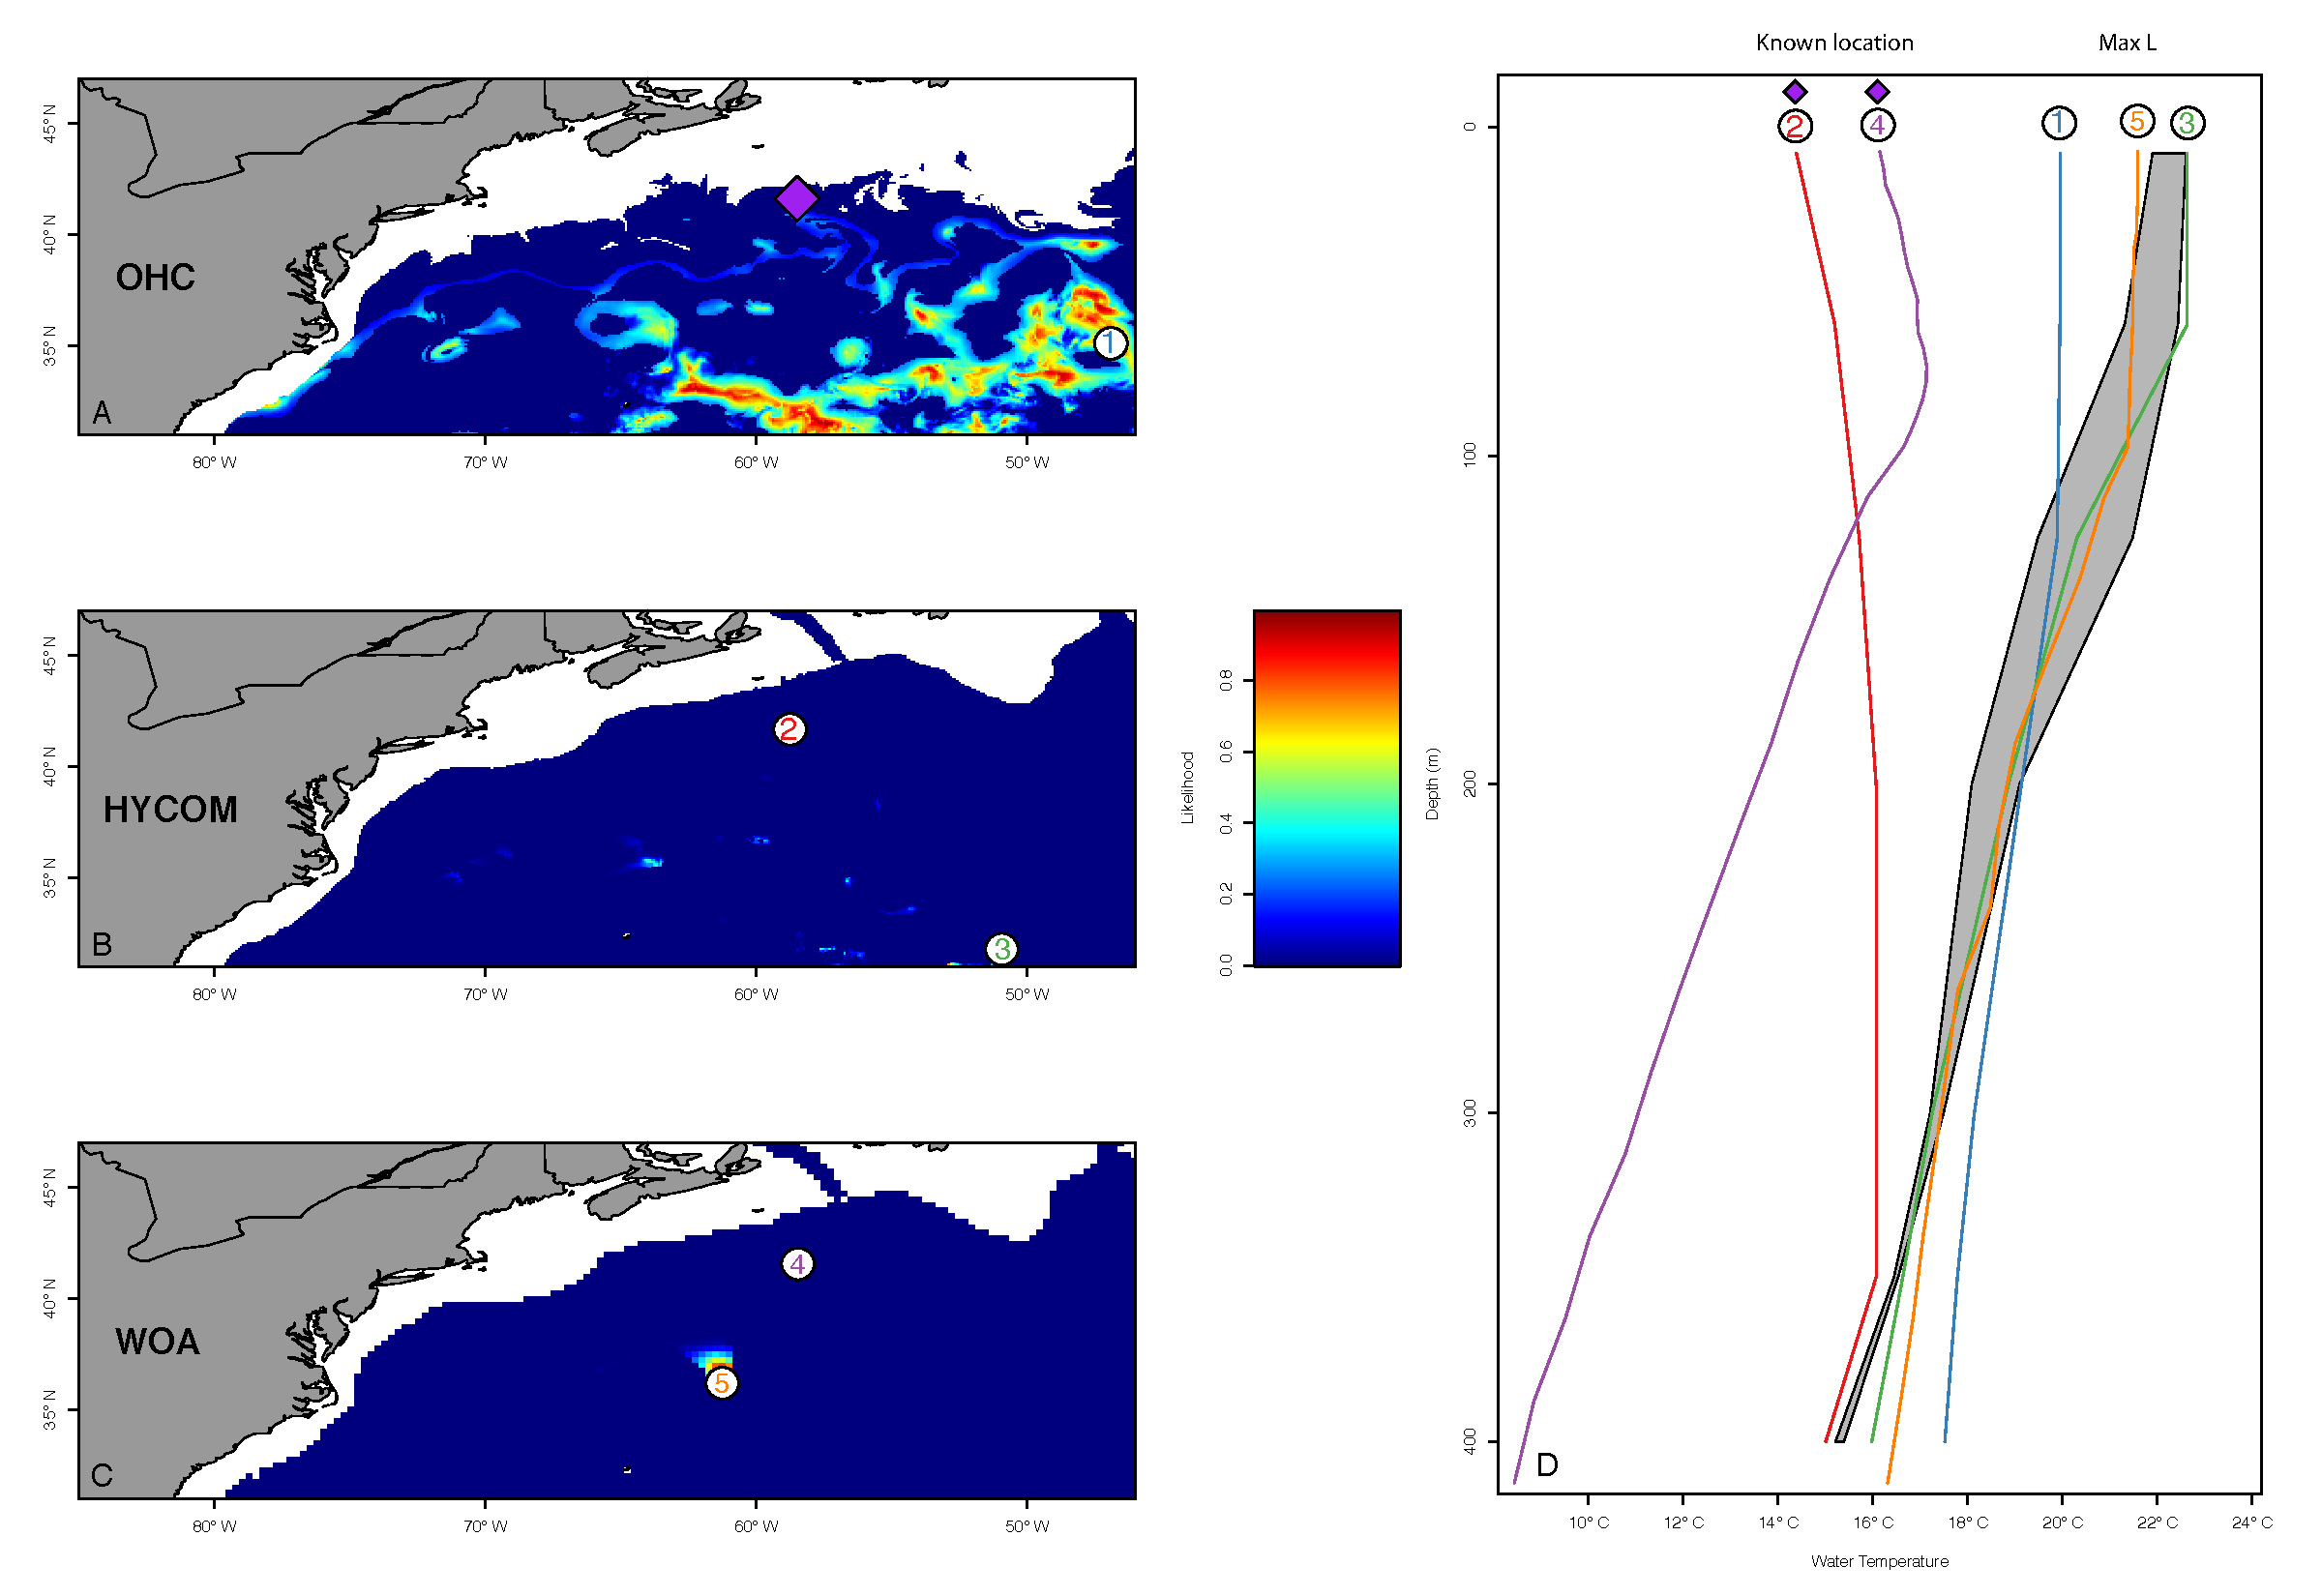
\includegraphics[width=8in]{images/A1_Fig5.pdf}
\caption[Example depth-temperature profile-based likelihoods]{Example depth-temperature profile-based likelihoods for ocean heat content (OHC), HYCOM and World Ocean Atlas (WOA)(panels A-C) for a given day of observation. Numbers correspond to the location where each depth-temperature profile (panel D) was taken. Purple diamond indicates known position for this example day. Profiles 2 and 4 correspond to profiles extracted from HYCOM and WOA, respectively, at the known location of the tag. In comparison, profiles 1, 3 and 5 indicate profiles taken from the grid cell containing the maximum likelihood, as calculated by HMMoce, for OHC, HYCOM and WOA, respectively. Grey shaded region in right panel indicates depth-temperature envelope measured by PSAT tag. This figure demonstrates an example day in which the measured PSAT tag data was compared to environmental grids to generate maximum likelihoods, but the resulting likelihoods exhibited significant error when compared to independent, known positions and profiles extracted at those locations.}
\label{fig:a1f5}
\end{figure}
\end{landscape}
\clearpage

%--------------------
%Figure a1f6:
\begin{figure}[p]
\centering
\includegraphics[width=.85\textwidth]{images/A1_Fig6.pdf}
\caption[Calculated \texttt{HMMoce} tracks and behavior for blue shark 141254]{Movements (A) and behavior (B) calculated using \texttt{HMMoce} for blue shark 141254. The tagged individual is considered resident where probability of residency is greather than 0.5 (grey points and bars in panels A and B, respectively). Green and red points indicate tag and pop-up location respectively. Black line follows predicted daily locations of tagged shark.}
\label{fig:a1f6}
\end{figure}
\clearpage

%--------------------
%Figure a1f7:
\begin{figure}[p]
\centering
\includegraphics[width=.85\textwidth]{images/A1_Fig7.pdf}
\caption[Calculated \texttt{HMMoce} tracks and behavior for blue shark 141256]{Movements (A) and behavior (B) calculated using \texttt{HMMoce} for blue shark 141256. The tagged individual is considered resident where probability of residency is greather than 0.5 (grey points and bars in panels A and B, respectively). Green and red points indicate tag and pop-up location respectively. Black line follows predicted daily locations of tagged shark.}
\label{fig:a1f7}
\end{figure}
\clearpage

%--------------------
%Figure a1f8:
\begin{figure}[p]
\centering
\includegraphics[width=.85\textwidth]{images/A1_Fig8.pdf}
\caption[Calculated \texttt{HMMoce} tracks and behavior for blue shark 141259]{Movements (A) and behavior (B) calculated using \texttt{HMMoce} for blue shark 141259. The tagged individual is considered resident where probability of residency is greather than 0.5 (grey points and bars in panels A and B, respectively). Green and red points indicate tag and pop-up location respectively. Black line follows predicted daily locations of tagged shark.}
\label{fig:a1f8}
\end{figure}
\clearpage

%--------------------
%--------------------
\section{Supplemental Tables}
%--------------------
%--------------------
%\vspace{-40mm}

% Table a1t1


\begin{table}[htbp]
\caption[Example error metrics for \texttt{HMMoce} model runs using different observation likelihoods]{Example error metrics for a HMMoce model run of each observation likelihood input: light (L), SST (S), ocean heat content (O), World Ocean Atlas profiles (W) and HYCOM profiles (H). Root-mean-square error (RMSE) is shown for Latitude, Longitude in degrees. Reported mean and standard deviation values are based on pointwise distance calculations from known positions (km). P1 and P2 indicate the calculated probability of state-switching from the Expectation-Maximization algorithm where, in this case, P1 is the probability of remaining in a migratory state (implemented in a migratory movement kernel for the convolution). P2 represents a resident behavior state. Migratory speeds were fixed at 2 m/s on a 0.08$^{\circ}$ grid for the example run.}
\label{tab:a1t1}
\centering
\resizebox{.7\textwidth}{!}{% <------ Don't forget this %
\begin{tabular}[t]{llllrrrr}
\toprule
\textbf{Species} & \textbf{PTT} & \textbf{Input} & \textbf{RMSE} & \textbf{Mean} & \textbf{SD} & \textbf{P1} & \textbf{P2}\\
\midrule
BSH & 141254 & LS & 1.52, 0.96 & 143.5 & 123.3 & 0.97 & 0.86\\
 &  & LO & 3.09, 1.03 & 265.0 & 238.1 & 0.94 & 0.78\\
 &  & LW & 2.59, 2.52 & 303.9 & 199.6 & 0.98 & 0.82\\
 &  & LH & 3.09, 1.43 & 285.7 & 229.5 & 0.97 & 0.84\\
 &  & LSO & 1.21, 0.81 & 117.8 & 96.8 & 0.94 & 0.83\\
 &  & LSW & 2.37, 2.73 & 288.4 & 209.1 & 0.96 & 0.69\\
 &  & LSH & 2.05, 1.2 & 186.0 & 168.7 & 0.98 & 0.86\\
\addlinespace
BSH & 141256 & LS & 0.42, 1.08 & 88.7 & 66.5 & 0.98 & 0.90\\
 &  & LO & 1.7, 1.03 & 169.1 & 132.9 & 0.97 & 0.83\\
 &  & LW & 1.23, 5.38 & 444.7 & 320.4 & 0.98 & 0.73\\
 &  & LH & 0.59, 1.15 & 109.4 & 64.9 & 0.96 & 0.83\\
 &  & LSO & 1.14, 2.61 & 190.0 & 216.8 & 0.96 & 0.76\\
 &  & LSW & 0.93, 4.67 & 353.6 & 302.8 & 0.99 & 0.86\\
 &  & LSH & 0.55, 1.03 & 91.4 & 68.2 & 0.95 & 0.81\\
\addlinespace
BSH & 141259 & LS & 1.87, 1.31 & 196.7 & 140.0 & 0.99 & 0.82\\
 &  & LO & 2.77, 1.17 & 277.4 & 173.9 & 0.99 & 0.82\\
 &  & LW & 5.71, 1.67 & 525.4 & 391.5 & 0.96 & 0.71\\
 &  & LH & 2.37, 1.55 & 252.9 & 160.9 & 0.97 & 0.69\\
 &  & LSO & 2.01, 1.31 & 206.8 & 149.1 & 0.98 & 0.73\\
 &  & LSW & 2.52, 1.87 & 284.2 & 170.9 & 0.99 & 0.80\\
 &  & LSH & 2, 1.36 & 206.8 & 154.0 & 0.98 & 0.67\\
\addlinespace
MKO & 141257 & LS & 0.79, 1.77 & 132.4 & 119.5 & 0.93 & 0.94\\
 &  & LO & 1.81, 2.03 & 225.0 & 148.6 & 0.94 & 0.92\\
 &  & LW & 2.29, 2.33 & 284.9 & 164.4 & 0.95 & 0.78\\
 &  & LH & 1.26, 2.22 & 171.3 & 170.7 & 0.91 & 0.88\\
 &  & LSO & 0.82, 1.58 & 123.8 & 109.9 & 0.94 & 0.95\\
 &  & LSW & 1.72, 2.29 & 231.5 & 158.6 & 0.95 & 0.85\\
 &  & LSH & 1.08, 2.03 & 147.8 & 158.8 & 0.93 & 0.93\\
\bottomrule
  \end{tabular}% <------ Don't forget this %
  }
\end{table}

% Table a1t2
\begin{table}
\caption[\texttt{HMMoce} model fit metrics, grid resolution and computation time]{Fit metrics and computation time (in mins) using an Amazon EC2 instance with 2.3GHz processors and 64 CPUs (High-performance computing; HPC) and a consumer-grade desktop computer with 2.53GHz processors and 4 CPUs (personal computer; PC) for blue shark 141256. The L row indicates total run time for calculating individual likelihoods from light (0.25$^{\circ}$ resolution), sea surface temperature (0.25$^{\circ}$), ocean heat content (0.08$^{\circ}$) and HYCOM 3D profiles (0.08$^{\circ}$) in the native resolution for each input environmental dataset. Environmental grids spanned 43$^{\circ}$ of longitude and 45$^{\circ}$ of latitude for this individual, resulting in a 539x564 matrix for daily OHC grids and daily HYCOM grids at each depth level (up to 35 depth levels to 1500m depth) and 173x181 matrix for daily SST and light grids. The following rows indicate computation time for one complete iteration of the HMM (including filtering, smoothing and parameter estimation) computed at each resolution listed. The HMM computations are performed after the observation likelihoods have been calculated. Resolution is the grid resolution in degrees. Reported metrics are based on pointwise distance calculations from known positions. Mean and standard deviation (SD) are in kilometers and root-mean-square error is for Latitude, Longitude in degrees.}

\label{tab:a1t2}
\centering
\begin{tabular}[t]{lrrrrrr}
\toprule
\textbf{Resolution} & \textbf{HPC Time} & \textbf{PC Time} & \textbf{Mean} & \textbf{SD} & \textbf{\texorpdfstring{RMSE\textsubscript{lat}}{RMSElat}
} & \textbf{\texorpdfstring{RMSE\textsubscript{lon}}{RMSElon}}\\
\midrule
L & 34.80 & 158.7 &  &  &  & \\
\addlinespace
0.08 & 23.90 & 1082.2 & 89.09 & 69.54 & 0.53 & 1.03\\
0.25 & 8.08 & 148.2 & 117.81 & 118.78 & 0.48 & 1.61\\
0.5 & 6.07 & 74.6 & 401.36 & 425.06 & 4.80 & 2.26\\
0.75 & 5.52 & 20.3 & 867.37 & 453.36 & 5.16 & 6.95\\
1 & 5.19 & 18.2 & 991.88 & 538.98 & 7.52 & 7.66\\
\bottomrule
\end{tabular}
\end{table}
